\documentclass[../main.tex]{subfiles}

% \title{Ray tracing}
% \date{2018-02-06}
% \author{Hongjie Lu}

\begin{document}

	% \maketitle
	% \pagenumbering{gobble}
	% \newpage
	\section{Ray tracing}
	\subsection{Introduction}
	\begin{figure}[h!]
	  \centering
	  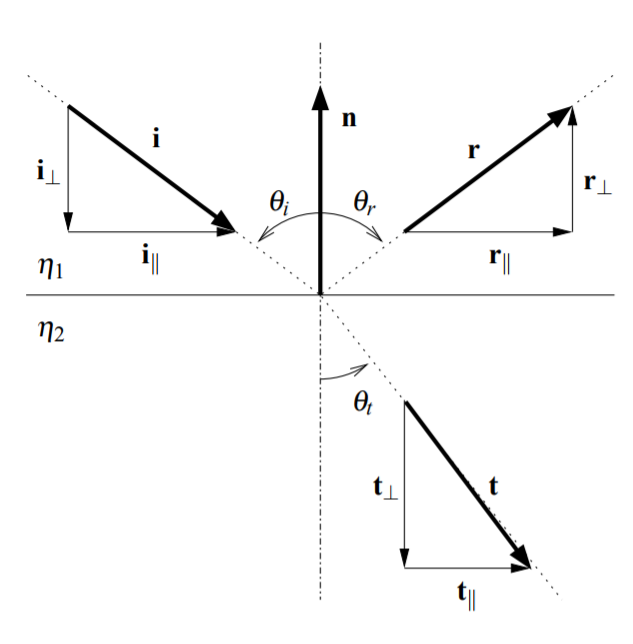
\includegraphics[scale=0.7]{../graphics/Ray_tracing1.png}
	  \caption{Scheme}
	  \label{fig:interface1}
	\end{figure}
	In the figure we have a interface between two materials with different refractive indices $n_1$ and $n_2$. The direction vector of the incident ray is \textbf{i} and we assume this vector is normalized. The normalized direction vectors of the reflected and transmitted rays are \textbf{r} and \textbf{t} and will be calculated. The normal vector \textbf{n}, orthogonal to the interface and pointing towards the first material $n_1$.
	\begin{equation}
	\abs{\textbf{i}}=\abs{\textbf{r}}=\abs{\textbf{t}}=\abs{\textbf{n}}
	\end{equation}
	The direction vectors of the rays can be split in components orthogonal and parallel to the interface. Taking the generic vector \textbf{v}, we have
	\begin{align}
	&\textbf{v}_{\perp}=\frac{\textbf{v}\cdot\textbf{n}}{\abs{\textbf{n}}^2}\textbf{n}=(\textbf{v}\cdot\textbf{n})\textbf{n}\\
	&\textbf{v}_{\parallel}=\textbf{v}-\textbf{v}_{\perp}\\
	&\abs{\textbf{v}}^2=\abs{\textbf{v}_{\parallel}}^2+\abs{\textbf{v}_{\perp}}^2\\
	&\cos\theta_v=\frac{\abs{\textbf{v}_{\perp}}}{\abs{\textbf{v}}}=\abs{\textbf{v}_{\perp}}\label{eq1}\\
	&\sin\theta_v=\frac{\abs{\textbf{v}_{\parallel}}}{\abs{\textbf{v}}}=\abs{\textbf{v}_{\parallel}}\label{eq2}
	\end{align}
	\subsection{Reflection}
	According to the law of reflection $\theta_r=\theta_i$, and \ref{eq1} \ref{eq2}, thus
	\begin{align}
	&\abs{\textbf{r}_{\perp}}=\cos\theta_r=\cos\theta_i=\abs{\textbf{i}_{\perp}}\\
	&\abs{\textbf{r}_{\parallel}}=\sin\theta_r=\sin\theta_i=\abs{\textbf{i}_{\parallel}}\\
	&\textbf{r}=\textbf{r}_{\parallel}+\textbf{r}_{\perp}=\textbf{i}_{\parallel}-\textbf{i}_{\perp}=\textbf{i}-2\textbf{i}_{\perp}=\textbf{i}-2(\textbf{i}\cdot\textbf{n})\textbf{n}
	\end{align}
	And we can find that the reflection vector \textbf{r} is also nomarlized.
	\subsection{Refraction}
	According to Snell's Law for the refraction case,
	\begin{equation}
	n_1\sin\theta_i=n_2\sin\theta_t\label{eq3}
	\end{equation}
	We leave out the total internal reflection case first here. With equations \ref{eq1} \ref{eq2}, we have
	\begin{align}
	&n_1\abs{\textbf{i}_{\parallel}}=n_2\abs{\textbf{t}_{\parallel}}\\
	&\textbf{t}_{\parallel}=\frac{n_1}{n_2}{\textbf{i}_{\parallel}}=\frac{n_1}{n_2}(\textbf{i}+\cos\theta_i\textbf{n})\\
	&\textbf{t}_{\perp}=-\sqrt{1-\abs{\textbf{t}_{\parallel}}^2\textbf{n}}\\
	&\textbf{t}=\textbf{t}_{\parallel}+\textbf{t}_{\perp}=\frac{n_1}{n_2}\textbf{i}+\left(\frac{n_1}{n_2}\cos\theta_i-\sqrt{1-\abs{\textbf{t}_{\parallel}}^2}\right)\textbf{n}=\frac{n_1}{n_2}\textbf{i}+\left(\frac{n_1}{n_2}\cos\theta_i-\sqrt{1-\sin^2\theta_t}\right)\textbf{n}
	\end{align}
	With \ref{eq3}, the refraction vector \textbf{t} can be conducted.
	\begin{figure}[h!]
	  \centering
	  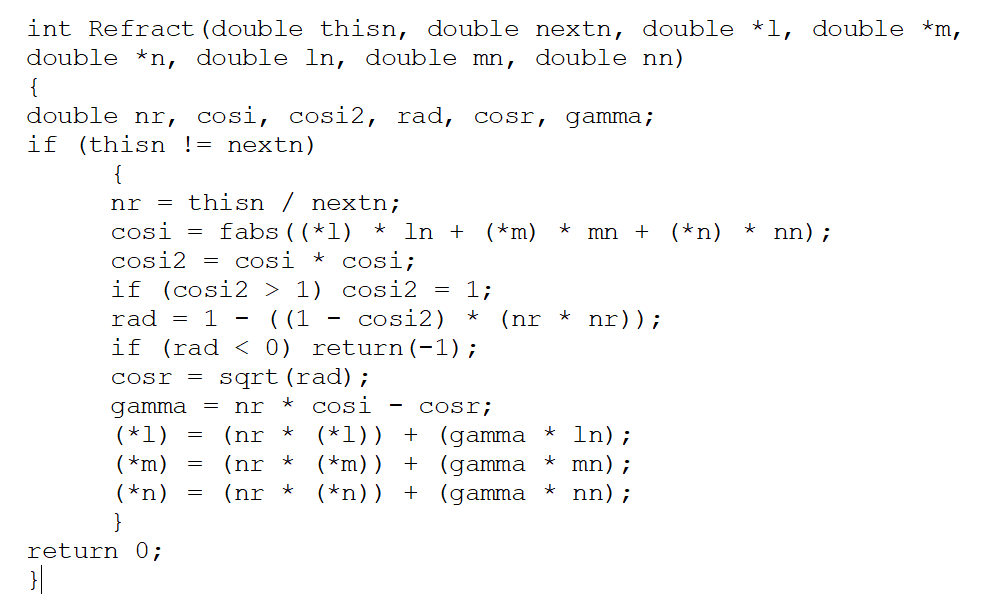
\includegraphics[scale=0.5]{../graphics/Ray_tracing2.png}
	  \caption{Refraction code in ZEMAX dll file}
	  \label{fig:Refraction}
	\end{figure}	
	\subsection{Reference}
	\url{https://graphics.stanford.edu/courses/cs148-10-summer/docs/2006--degreve--reflection_refraction.pdf}
	\section{Real ray tracing}
	Here the term real ray tracing refers to the 'case 5' part of the ZEMAX DLL file.\\
	The real ray trace portion of the DLL, type code 5, allows definition of the surface transmittance. The surface transmittance must be a number between 0.0 and 1.0, and indicates the relative fraction of intensity that the ray transmits through the surface. In this context, transmit means "continues on", so for reflective surfaces, the transmitted portion is that which normally reflects to the next surface.\\
	In standard dll file, real ray tracing calculates the intersection point $(x,y,z)$ of the sag surface and the ray with the direction vector $(l,m,n)$, and the normal vector (ln,mn,nn) at this point.\\
	\subsection{Intersection}
	With the ray starting point $\textbf{O}=(x_0,y_0,z_0)$ and the normalized ray direction vector $\textbf{D}=(l,m,n)$, we can express the ray $\textbf{P}=(x,y,z)$ in parametric form
	\begin{align}
	&\textbf{P}=\textbf{O}+t\textbf{D}\\
	&\left\{
		\begin{array}{ll}
		x=x_0+tl\\
		y=y_0+tm\\
		z=z_0+tn
		\end{array}
		\right.\label{eq4}
	\end{align}
	We can first transform the surface sag equation into another form:
	\begin{align}
	&z=\frac{c\rho^2}{1+\sqrt{1-(1+K)c^2\rho^2}}\\
	&\rho^2+(1+K)z^2-\frac{2z}{c}=0\\
	&where\ \rho^2=x^2+y^2
	\end{align}
	To find the intersection between this surface and an arbitrary ray, substitute the ray equation in the surface equation:
	\begin{align}
	&(x_0+tl)^2+(y_0+tm)^2+(1+K)(z_0+tn)^2=\frac{2(z_0+tn)}{c}\\
	&(l^2+m^2+n^2(1+K))t^2+2\left(x_0l+y_0m+(1+K)z_0n-\frac{n}{c}\right)t+(x_0^2+y_0^2+z_0^2(1+K)-\frac{2z_0}{c})=0
	\end{align}
	Because the ray direction vector is normalized, so we have $l^2+m^2+n^2=1$. And if we assume the ray start point satifies $z_0=0$, the equation can be simplifed as
	\begin{align}
	&(1+n^2K)t^2+2\left(x_0l+y_0m-\frac{n}{c}\right)t+(x_0^2+y_0^2)=0\\
	&choose	\left\{
				\begin{array}{ll}
				a_1=a=(1+n^2K)\\
				b_1=-\frac{b}{2}=\frac{n}{c}-x_0l-y_0m\\
				c_1=c=x_0^2+y_0^2
				\end{array}
				\right.
	\end{align}
	Here we choose $a_1$, $b_1$ and $c_1$ which ar econsistent with that in ZEMAX DLL file 'case 5' part. Therefore the solution is 
	\begin{equation}
	t=\frac{-b\pm\sqrt{b^2-4ac}}{2a}=\frac{b_1\pm\sqrt{b_1^2-a_1c_1}}{a_1}=\frac{c_1}{b_1\mp\sqrt{b_1^2-a_1c_1}}
	\end{equation}
	We then can calculate the intersection using equation \ref{eq4}
	\subsection{Normal vector}
	First, we will derive the normal vector form of an arbitrary point on an arbitrary surface. We consider the surface $U(x,y,z)=k$, it is said to be smooth if the gradient $\nabla{U}=\langle U_x,U_y,U_z \rangle$ is continuous and non-zero at any point on the surface. Equivalently, we ofter write:
	\begin{align}
	&\nabla{U}=U_x\textbf{e}_x+U_y\textbf{e}_y+U_z\textbf{e}_z\\
	&where\ \textbf{e}_x=\langle 1,0,0 \rangle,\textbf{e}_y=\langle 0,1,0 \rangle,\textbf{e}_z=\langle 0,0,1 \rangle
	\end{align}
	Suppose that $\textbf{r}(t)=\langle x(t),y(t),z(t) \rangle$ lies on a smooth surface $U(x,y,z)=k$. Applying the derivative with respect to t to both sides of the equation of the surface yields
	\begin{align}
	&\frac{dU}{dt}=\frac{d}{dt}k=0\\
	&\nabla{U}\cdot\textbf{v}=0\\
	&where \textbf{v}=\langle x'(t),y'(t),z'(t) \rangle
	\end{align}
	\textbf{v} is tangent to the surface because it is tangent to a curve on the surface, which implies that $\nabla{U}$ is orthogonal to each tangent vector \textbf{v} at a given point on the surface. We thus say that the gradient $\nabla{U}$ is normal to the surface $U(x,y,z)=k$ at each point on the surface. To get the normalized normal vector, we can simply divide the gradient $\nabla{U}$ with its length.\\  
	Have known the way to calculate the normal vector, we come back to our case, where we want to calculate the normal vector at the intersection point that we have already got in the former part.
	\begin{align}
	&U(x,y,z)=\rho^2+(1+K)z^2-\frac{2z}{c}=0\\
	&\frac{dU}{d\rho}=2\rho\\
	&\Rightarrow \frac{dU}{dx}=2x, \frac{dU}{dy}=2y\\
	&\frac{dU}{dz}=2(1+K)z-\frac{2}{c}\\
	\abs{U}&=\sqrt{\left(\frac{dU}{dx}\right)^2+\left(\frac{dU}{dy}\right)^2+\left(\frac{dU}{dz}\right)^2}\\
	&=\sqrt{4\rho^2+4\left((1+K)z-\frac{1}{c}\right)^2}\\
	&=2\sqrt{-(1+K)z^2+\frac{2z}{c}+\left((1+K)z-\frac{1}{c}\right)^2}\\
	&=2\sqrt{K(1+K)z^2-\frac{2k}{c}z+\frac{1}{c^2}}\\
	&=\frac{2}{c}\sqrt{K(1+K)c^2z^2-2kcz+1}
	\end{align}
	And we can get the normalized normal vector by diveding the $\nabla{U}=\langle U_x,U_y,U_z \rangle$ with its length $\abs{U}$, which is consistent with the code in DLL file.
	\begin{figure}[h!]
	  \centering
	  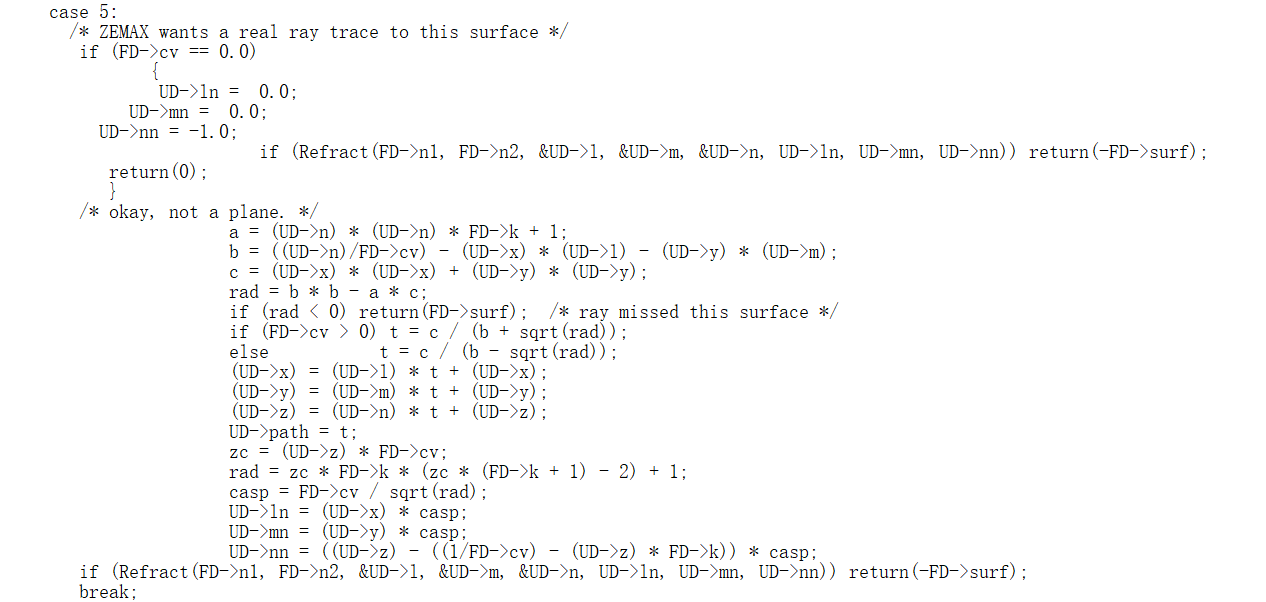
\includegraphics[scale=0.6]{../graphics/Ray_tracing3.png}
	  \caption{Real ray tracing code in ZEMAX dll file 'case 5'}
	  \label{fig:realraytracing}
	\end{figure}
	\subsection{Reference}
	ZEMAX manual-Chapter11(SurfaceType)-UserDefined\\
	\url{https://www.cl.cam.ac.uk/teaching/1999/AGraphHCI/SMAG/node2.html}\\
	\url{https://www.scratchapixel.com/lessons/3d-basic-rendering/minimal-ray-tracer-rendering-simple-shapes/ray-sphere-intersection}\\
	\url{http://math.etsu.edu/multicalc/prealpha/chap3/chap3-6/printversion.pdf}



	\end{document}
	